O maior diferencial do conversor Boost é a capacidade de elevar a tensão a partir da corrente na entrada. A figura \ref{cboost} ilustra o circuito simplificado de um conversor Boost.

\begin{figure}[h]
\center
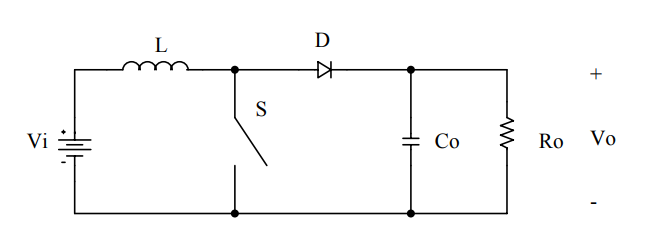
\includegraphics[scale=0.55]{imagens/circuito_boost.png}
\caption{Circuito simplificado do conversor Boost.}\label{cboost} 
\caption*{Fonte: Introdução aos conversores CC-CC (2001)}
\end{figure}

Durante a etapa de condução, com a chave $S$ fechada, o indutor $L$ é magnetizado pela alimentação. Nota-se que a chave age como um curto para a saída, que só é alimentada pelo capacitor $C_o$ uma vez que há o diodo $D$ impedindo que esse seja curto-circuitado pela chave. Quando a chave abre, o indutor e a fonte fornecem energia à saída e ao capacitor, dessa forma, elevando a tensão aparente na saída. O comportamento da tensão no indutor pode ser visto, de forma simplificada, na figura \ref{g1bo}.

\begin{figure}[h]
\center
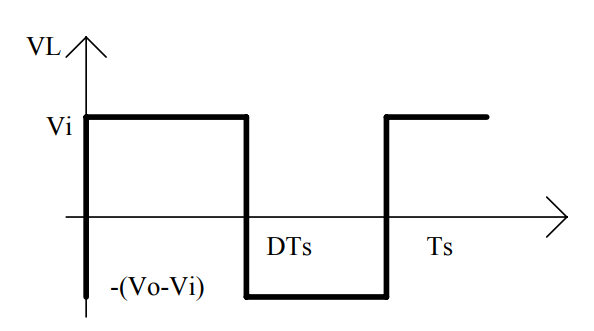
\includegraphics[scale=0.55]{imagens/grafico1_boost.png}
\caption{Comportamento da tensão no indutor de um conversor Boost.}\label{g1bo} 
\caption*{Fonte: Introdução aos conversores CC-CC (2001)}
\end{figure}

Assumindo, com idealidades, que a tensão média sobre o indutor é nula, temos \[
V_o = \frac{1}{T_{s}}\int_{o}^{DT_{s}}V_{i}dt =  \frac{1}{T_{s}}\int_{o}^{(1-D)T_{s}}(V_{o} - V_{i})dt
\] \[
\implies \frac{V{o}}{V{i}} = \frac{1}{1-D}
.\]

A relação entre a razão cíclica e o ganho estático pode ser vista na figura \ref{g2bo}.

\begin{figure}[h]
\center
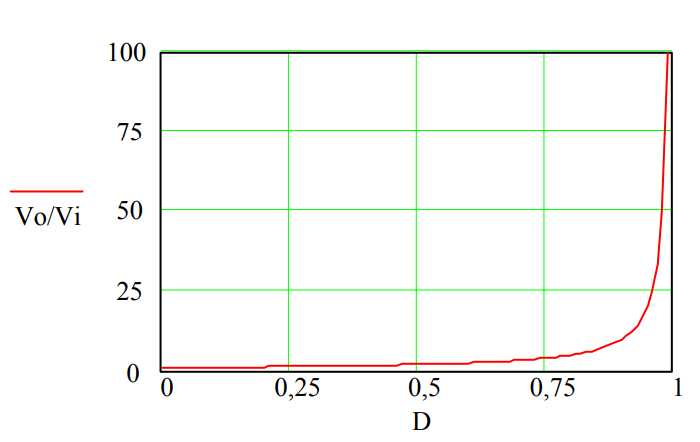
\includegraphics[scale=0.55]{imagens/grafico2_boost.png}
\caption{Relação entre o ganho estático e a razão cíclica em um conversor Boost.}\label{g2bo} 
\caption*{Fonte: Introdução aos conversores CC-CC (2001)}
\end{figure}

O comportamento da tensão e da corrente nos componentes do conversor Boost é ilustrada na figura \ref{g3bo}.

\begin{figure}[h]
\center
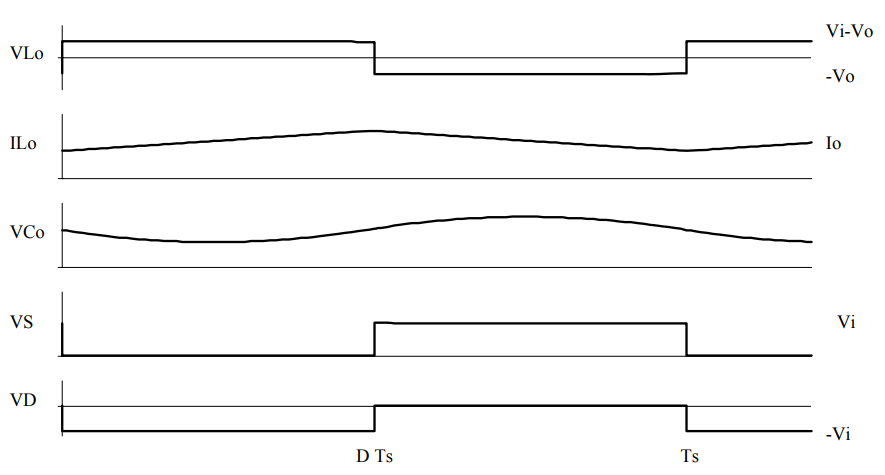
\includegraphics[scale=0.55]{imagens/grafico3_boost.png}
\caption{Tensão e corrente nos componentes do conversor Boost.}\label{g3bo} 
\caption*{Fonte: Introdução aos conversores CC-CC (2001)}
\end{figure}

As principais características do conversor Boost são sua capacidade de aumentar a tensão da saída, apesar de fornecer corrente de forma descontínua, e baixa distorção da corrente consumida da alimentação.

